\documentclass[conference]{IEEEtran}

\usepackage{amsmath}
\usepackage{dsfont}
\newcommand{\1}{\mathds{1}}
\newcommand{\E}{\mathrm{E}}
\usepackage{booktabs}
\usepackage[flushleft]{threeparttable}
\newcommand{\mynote}{\item \leavevmode\kern-\scriptspace\kern-\labelsep}
\usepackage{graphicx}
\usepackage{hyperref}
\usepackage[numbers]{natbib}
\usepackage{flushend}
\newcommand{\myrotate}[1]{\rotatebox[origin=c]{90}{#1}}
\newcommand{\PreserveBackslash}[1]{\let\temp=\\#1\let\\=\temp}
\newcommand{\mycell}[1]{\parbox[m]{1.1in}{\PreserveBackslash\raggedright #1}}
\usepackage{multirow}

\title{
  Stack Overflow Badges and User Behavior: \\
  An Econometric Approach
}
\author{
  Andrew Marder \\
  Harvard Business School \\
  Boston, Massachusetts, USA \\
  \href{mailto:amarder@hbs.edu}{amarder@hbs.edu}
}
\date{\today}

\clubpenalty = 10000
\widowpenalty = 10000
\displaywidowpenalty = 10000

\begin{document}

\maketitle

\begin{abstract}
Let's work in Kraft and Todd to frame this paper.

What motivates individuals to work? @Ellingsen summarize a growing body of research on behavioral agency theory. In the classical principal-agent model, a principal motivates an agent to exert effort in exchange for material goods. Behavioral agency theory, explores how agents may derive utility from how they are perceived by others - in addition to the utility derived from material benefits. In fact, @Frey1997 provide an empirical example where the net benefit of a monetary reward is negative.

The theoretical literature considers a variety of research questions. @Frey explores how a principal can use awards to compensate agents. He develops a number of hypotheses describing the conditions under which awards are more or less likely to be used as compensation. @Moldovanu develop a theoretical model to describe the optimal use of awards by an award-granting organization. They derive the optimal award strategy to maximize organization output, and describe how the classes and number of awards changes as the distribution of agent abilities and preferences changes. @Kraft-Todd give a general overview of how to promote cooperation in the field They group interventions to promote cooperation into four categories:

*   Cost-benefit interventions (mixed results)
    1. Material rewards - case or gifts provided in exchange for contributing
    2. Increased efficacy - matching/seed funds provided, or benefit to recipients emphasized
*   Social interventions (consistently effective)
    3. Observability - others informed about your contribution decisions
    4. Descriptive norms - you are informs about contribution decisions of others

There are a number of empirical papers measuring the impact of manipulating award systems. @Kosfeld run a randomized controlled trial, 7 control groups of about 10 students completed a data entry task for two hours, while 9 treatment groups performed the same task but the two students who put in the most effort were presented an non-monetary award publicly. The treatment group was about 12 percent more productive on average than the control group, and the difference in quality between the two groups was not statistically different from zero. @Ashraf run a randomized controlled trial to disentangle different award effects. In their setting, comparison between Community Health Assistants is discouraging for low-performing students. While recognition from the employer and social visibility are motivating. @Tran show that informing students of their rank in an English class increased effort and improved final outcomes. Individuals value high ranks even when those ranks cannot be reliably communicated to others. @Delfgaauw find a sales tournament with no monetary incentive is just as effective is equally effective at promoting sales as the same tournament with a cash prize. @Markham show that an award program recognizing good attendance records is effective at lowering absenteeism at one treatment plant compared to three control plants.

There are two empirical studies that lack obvious treatment and control groups. @Neckerman measure the impact of an award system on employee productivity at a call center of a Fortune 500 company. The small monetary award, given publicly, had a statistically significant effect on productivity in the month following receipt of the award. @Chan is an interesting observational study. They measure the impact of winning a prestigious academic award on one's publication record. Constructing a synthetic control group by matching award winners with similarly productive academics, they see how much research outcomes diverge for winners of the award with similarly qualified individuals that did not win the award.
\end{abstract}

\section{Introduction}

Stack Overflow is a question and answer community designed for programmers. It is the largest of 130 communities in the Stack Exchange network. Created in 2008, the knowledge organized by Stack Overflow has become a valuable resource for software developers. On January 20, \citet{Spoelsky2015} announced that Stack Exchange had raised \$40 million in venture capital funding. Stack Overflow gives users who ask questions access to expert technical help, while users who answer questions build their reputation for technical expertise, a good reputation can be used to find better employment opportunities.

\citet{Deterding2011} define ``\textit{gamification} as the use of game design elements in non-game contexts.'' Stack Overflow gamifies the process of asking and answering questions as follows. A user earns reputation points when another user votes on her posts (5 points when a question is voted up, 10 points when an answer is voted up, 15 points when an answer is accepted, and 2 points when an edit is approved). As a user earns reputation points she unlocks privileges on the site. For instance, a user must have at least 15 reputation points to vote up a question or answer.\footnote{A full list of privileges and the corresponding reputation points is available at \url{http://stackoverflow.com/help/privileges}.} Users are awarded badges for special achievements. For example, one receives the \textit{Informed} badge by reading the tour page.\footnote{The Stack Overflow tour can be found at \url{http://stackoverflow.com/tour}, and all badges are listed on \url{http://stackoverflow.com/help/badges}.}

This paper takes a first step along the path of applying econometric analysis to publicly available Stack Overflow data. Do badges motivate users to contribute to the site? Which badges are most effective? What types of user contributions are responsive to gamification? To begin answering these questions, I study how users behave around the time they are awarded badges.

\section{Kraft-Todd}

\begin{table}
  \centering
  \caption{Summary of findings from \citet{Kraft-Todd}.}
  \label{tab:kraft-todd}
  \begin{tabular}{|c|c|c|}
    \cline{2-3}
\multicolumn{1}{c|}{} & \multicolumn{2}{c|}{} \\[-.05in]
\multicolumn{1}{c|}{} & \multicolumn{1}{c}{Material-benefit} & Social-benefit \\
\multicolumn{1}{c|}{} & \multicolumn{2}{c|}{} \\[-.07in]
    \hline
 & & \\
\myrotate{Self-interest} & \mycell{Material rewards \\ \\ Cash or gifts provided in exchange for contributing} & \mycell{Observability \\ \\ Others informed about your contribution decisions} \\
& & \\
    \cline{2-3}
& & \\
\myrotate{Other-interest} & \mycell{Increased efficacy \\ \\ Matching/seed funds provided, or benefit to others emphasized} & \mycell{Descriptive norms \\ \\ You are informed about contribution decisions of others} \\[5pt]
& & \\
    \hline
  \end{tabular}
\end{table}

\section{Methods}

\citet{Grant2013} present empirical evidence that three badges awarded for editing encourage recipients to make more edits in the two months preceding receipt of the badge compared to the two months after receiving the badge. This paper extends their findings by examining all types of user activity (posting questions, posting answers, and editing posts), and exploring the impact of three new badges awarded for asking questions. Table \ref{tab:badges} describes the six badges considered in this paper.


\begin{table}
  \begin{threeparttable}
    % \ra{1.2}
    \caption{Badges of interest}
    \label{tab:badges}
    \begin{tabular}{@{}llccc@{}}
      \toprule
      Name & Description & Awarded & Introduced & Dropped \\
      \midrule
      Strunk \& White & Edited 80 posts & 7,073 & 2008-09-15 & 0.00 \\
      Copy Editor & Edited 500 posts & 1,288 & 2010-07-09 & 0.04 \\
      Archaeologist & Edited 100 posts that were inactive for 6 months & 691 & 2011-08-15 & 0.05 \\
      Curious & Asked a well-received question on 5 separate days & 138,264 & 2014-07-02 & 0.86 \\
      Inquisitive & Asked a well-received question on 30 separate days & 14,081 & 2014-07-02 & 0.92 \\
      Socratic & Asked a well-received question on 100 separate days & 1,240 & 2014-07-02 & 0.93 \\
      \bottomrule
    \end{tabular}
    \begin{tablenotes}
    \item The six badges considered in this paper were introduced to the Stack Overflow site at different times. The Strunk \& White badge was first awarded on September 15, 2008, while the three badges for asking questions were all introduced on July 2, 2014. Since the badges for asking questions were added to the site so recently many users who have been awarded these badges earned them for actions taken before the badge was introduced. For instance, 86\% of users who earned the Curious badge were awarded the badge for actions taken before July 2, 2014. I drop these users from the analysis as they have no incentive to change their behavior to earn the Curious badge.
    \end{tablenotes}
  \end{threeparttable}
\end{table}


Let $y_{it}$ be the number of edits user $i$ makes on day $t$, and $t_i^*$ denote the day user $i$ receives the badge of interest. Following the approach of \citet{Jacobson1993}, I regress the number of edits user $i$ makes on day $t$ on a user fixed effect $\alpha_i$, a set of dummy variables indicating whether the user received the badge on day $t-k$, while controlling for day of the week effects $\gamma_j$

\begin{equation}
\begin{split}
\log(1 + y_{it}) = \; & \alpha_i + \sum_{k=-29}^{30} \1 \{ t = t_i^* + k \} \delta_k \; + \\
  & \sum_{j=1}^6 \1 \{ t \bmod 7 = j \} \gamma_j + \epsilon_{it}.
\end{split}
\end{equation}

The model parameters are estimated using an ordinary least squares regression, and standard errors are clustered at the user level. Define $f(k)$ to be the expected number of actions taken on the $k$'th day since receiving the badge

\begin{equation}
f(k) = \E \left[ \log(1 + y_{it}) \; | \; t=t^*_i + k \right].
\end{equation}

The predicted number of actions $\hat{f(k)}$ is presented in Figure \ref{fig:badges}. The 95\% confidence interval is depicted as a gray band around the linear prediction, standard errors were calculated using the delta method \citep{Williams2012}.

\section{Results}

\begin{figure*}
  \centering
  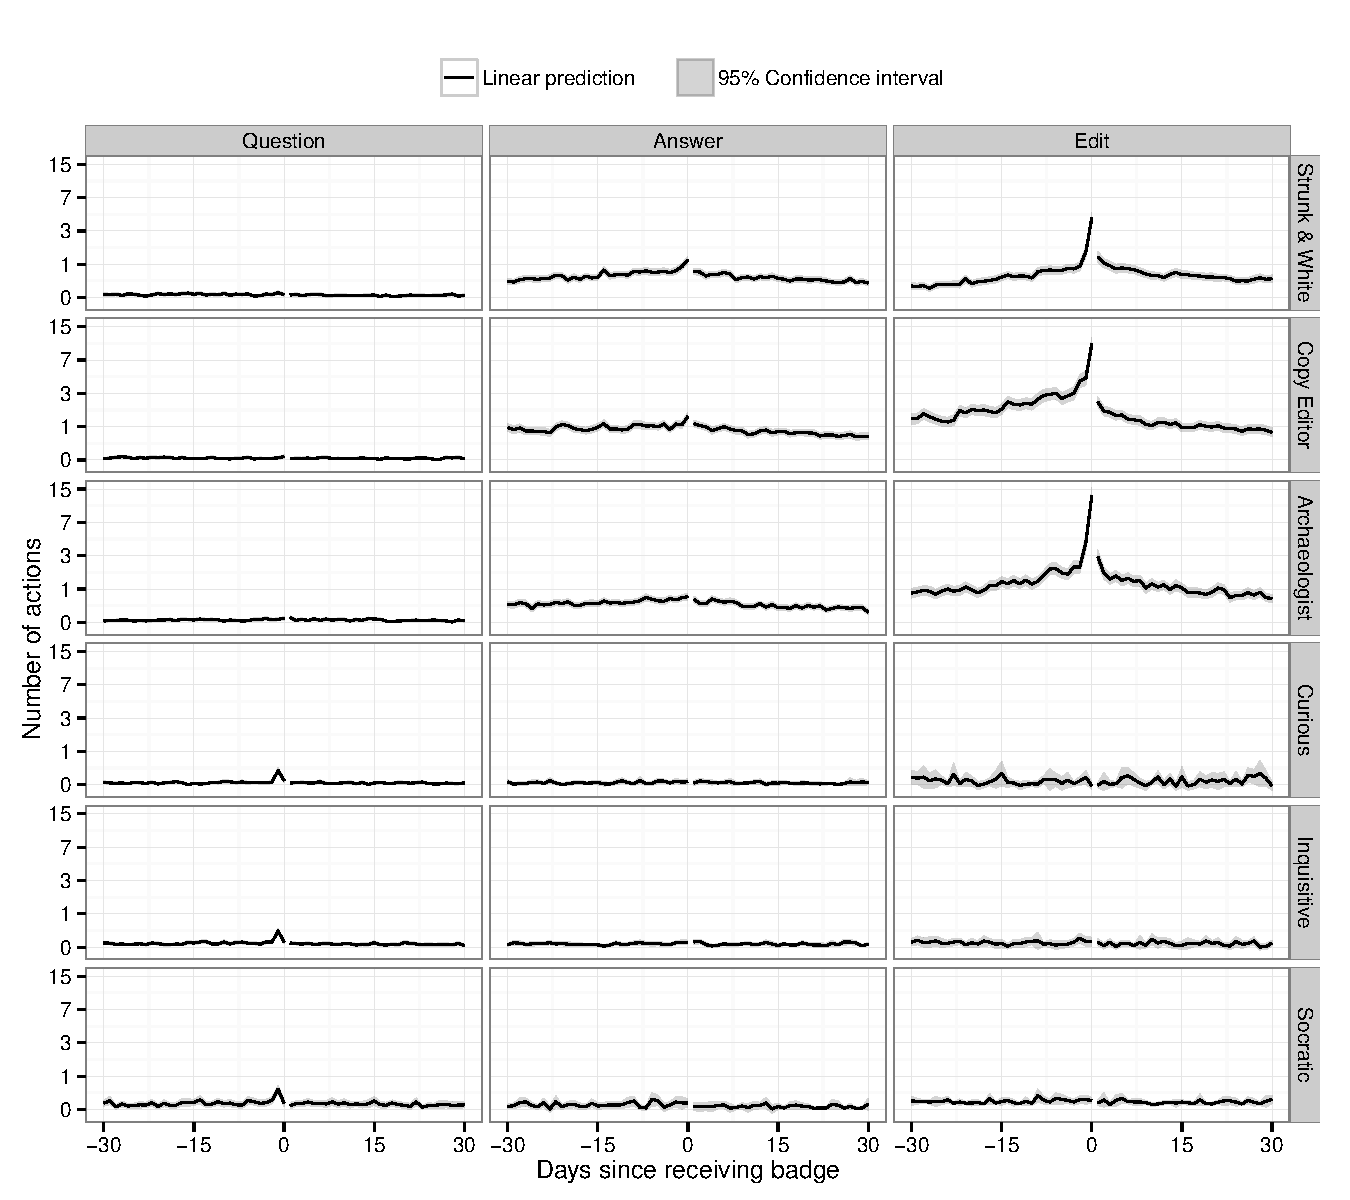
\includegraphics[width=\textwidth]{../figures/badges.pdf}
  \caption{User activity over time \label{fig:badges}}
\end{figure*}

The first three rows of Figure \ref{fig:badges} illustrate how user activity changes around the time one earns a badge for editing. Each row is labeled with the name of the focal badge (\textit{Strunk \& White}, \textit{Copy Editor}, and \textit{Archaeologist}). There is one column for each type of user action (posting a question, posting an answer, or editing a post). The figure confirms the findings of \citet{Grant2013}. Editing increases gradually before receiving a badge for editing, with a large jump in activity on the award day. We also see that editing drops quickly after receiving the badge and gradually declines over time. It's interesting to see how few questions were asked by the recipients of the editing badges, and to see that the rate of answering questions has a very slight increase leading up to receiving the badge and a similarly slight decrease after receiving the badge.

The results for the question-focused badges, \textit{Curious}, \textit{Inquisitive}, and \textit{Socratic}, are quite different. In general, recipients of these badges are not particularly active on the site. The average level of questions, answers, and edits made all hover near zero. The uptick in questions asked on the day before receiving the badge is mechanical. Many users who earn these badges ask a question the day before they earn the badge.

By looking at a new set of badges we find that not all badges are effective at motivating user activity. The three badges for editing seem effective at changing user behavior around the time the badge is awarded. The three badges for questions do not appear effective at changing user behavior.

\section{Conclusion}

When interpreting the empirical results of this paper, please consider Holland and Rubin's motto "no causation without manipulation" \citep{Holland1986}. There is no manipulation of the explanatory variable in this study, consequently we have not identified the causal effect of badges. To estimate the causal impact of badges on user activity we need to find a source of exogenous variation \citep{Miller2013}.

This paper confirms the empirical observation of \citet{Grant2013}, on average users who receive a badge for editing make more edits in the 30 days prior to receiving the badge compared to the 30 days after receiving the badge. In addition, we consider how other user actions respond to editing badges. The number of questions asked each day is near zero. Finally, we show that users who received badges for asking questions behaved differently. In particular, we found that users do not appear motivated to change their activity levels to earn badges for asking questions.

\section*{Acknowledgements}

The author would like to thank...

\nocite{Antin2011, MSRChallenge2015, se-dump}

\renewcommand{\bibfont}{\small}
\bibliographystyle{IEEEtranN}
\bibliography{IEEEabrv,clean}

\end{document}